\subsection{Unlocking the Magic of Sense Antennas!}

\begin{tcolorbox}[colback=gray!10, colframe=black, title=E9H08] What is the function of a sense antenna?
\begin{enumerate}[label=\Alph*.]
    \item \textbf{It modifies the pattern of a DF antenna to provide a null in only one direction}
    \item It increases the sensitivity of a DF antenna array
    \item It allows DF antennas to receive signals at different vertical angles
    \item It provides diversity reception that cancels multipath signals
\end{enumerate} \end{tcolorbox}

In radio communication, particularly within the context of Direction Finding (DF) systems, sense antennas play a crucial role. A sense antenna is specifically designed to enhance the direction-finding capabilities of a primary antenna (also known as the main or array antenna). The correct answer to the question is option A: It modifies the pattern of a DF antenna to provide a null in only one direction.

\subsubsection*{Related Concepts: :}

1. \textbf{Direction Finding (DF):}: DF is the process of determining the direction from which a received signal was transmitted. It's widely used in various fields, including aviation, maritime navigation, and military operations.

2. \textbf{Antenna Pattern:}: The radiation pattern of an antenna defines how the antenna radiates energy in various directions. A sense antenna can alter this pattern by creating regions of null, which helps in pinpointing the signal source's location.

3. \textbf{Null Direction:}: A null is an orientation where the antenna's sensitivity decreases to its minimum. By creating a null direction, sense antennas enable better localization of signals.

4. \textbf{Multipath Interference:}: It occurs when signals take multiple paths to reach the receiving antenna, causing distortion in the received signal. Some configurations of sense antennas can help mitigate the effects of multipath by adjusting the reception characteristics.

\subsubsection*{Calculation and Diagram:}

In practice, the performance of sense antennas can be analyzed using antenna theory and signal processing methods. For example, consider how we could analyze the effect of introducing a sense antenna in a DF system.

1. \textbf{Antenna Gain Calculation:}:
    - The gain of an antenna can be calculated using the following formula:
    \[
    G = \frac{4 \pi A_e}{\lambda^2}
    \]
    Where:
    - \(G\) is the antenna gain (dimensionless),
    - \(A_e\) is the effective aperture area (in square meters),
    - \(\lambda\) is the wavelength of the signal (in meters).

2. \textbf{Example Calculation:}:
    - Assume a sense antenna with an effective aperture area of \(A_e = 0.5 \, m^2\) at a frequency of 900 MHz.
    - Calculate the wavelength \(\lambda\) first:
    \[
    \lambda = \frac{c}{f}
    \]
    where \(c \approx 3 \times 10^8 \, m/s\) and \(f = 900 \times 10^6 \, Hz\).
    \[
    \lambda = \frac{3 \times 10^8}{900 \times 10^6} = 0.333 \, m
    \]
    - Now substitute the values into the gain formula:
    \[
    G = \frac{4 \pi (0.5)}{(0.333)^2} \approx 6.94
    \]

3. \textbf{Diagram:}:
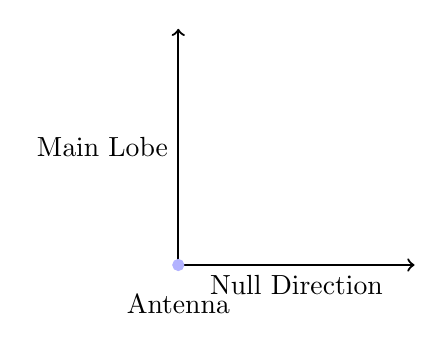
\begin{tikzpicture}
    \draw[->, thick] (0,0) -- (3,0) node[midway, below] {Null Direction};
    \draw[->, thick] (0,0) -- (0,3) node[midway, left] {Main Lobe};
    \filldraw[blue!30] (0,0) circle (2pt);
    \node at (0,-0.5) {Antenna};
\end{tikzpicture}

In summary, a sense antenna is integral in improving the performance of Direction Finding systems by modifying the angular response of the main antenna to create nulls in specific directions, essential for effective signal localization.
